        \clearpage
        \begin{figure*}[ht]
            \pdfbookmark[2]{ID 06}{figure_id_06}
        	\centering
            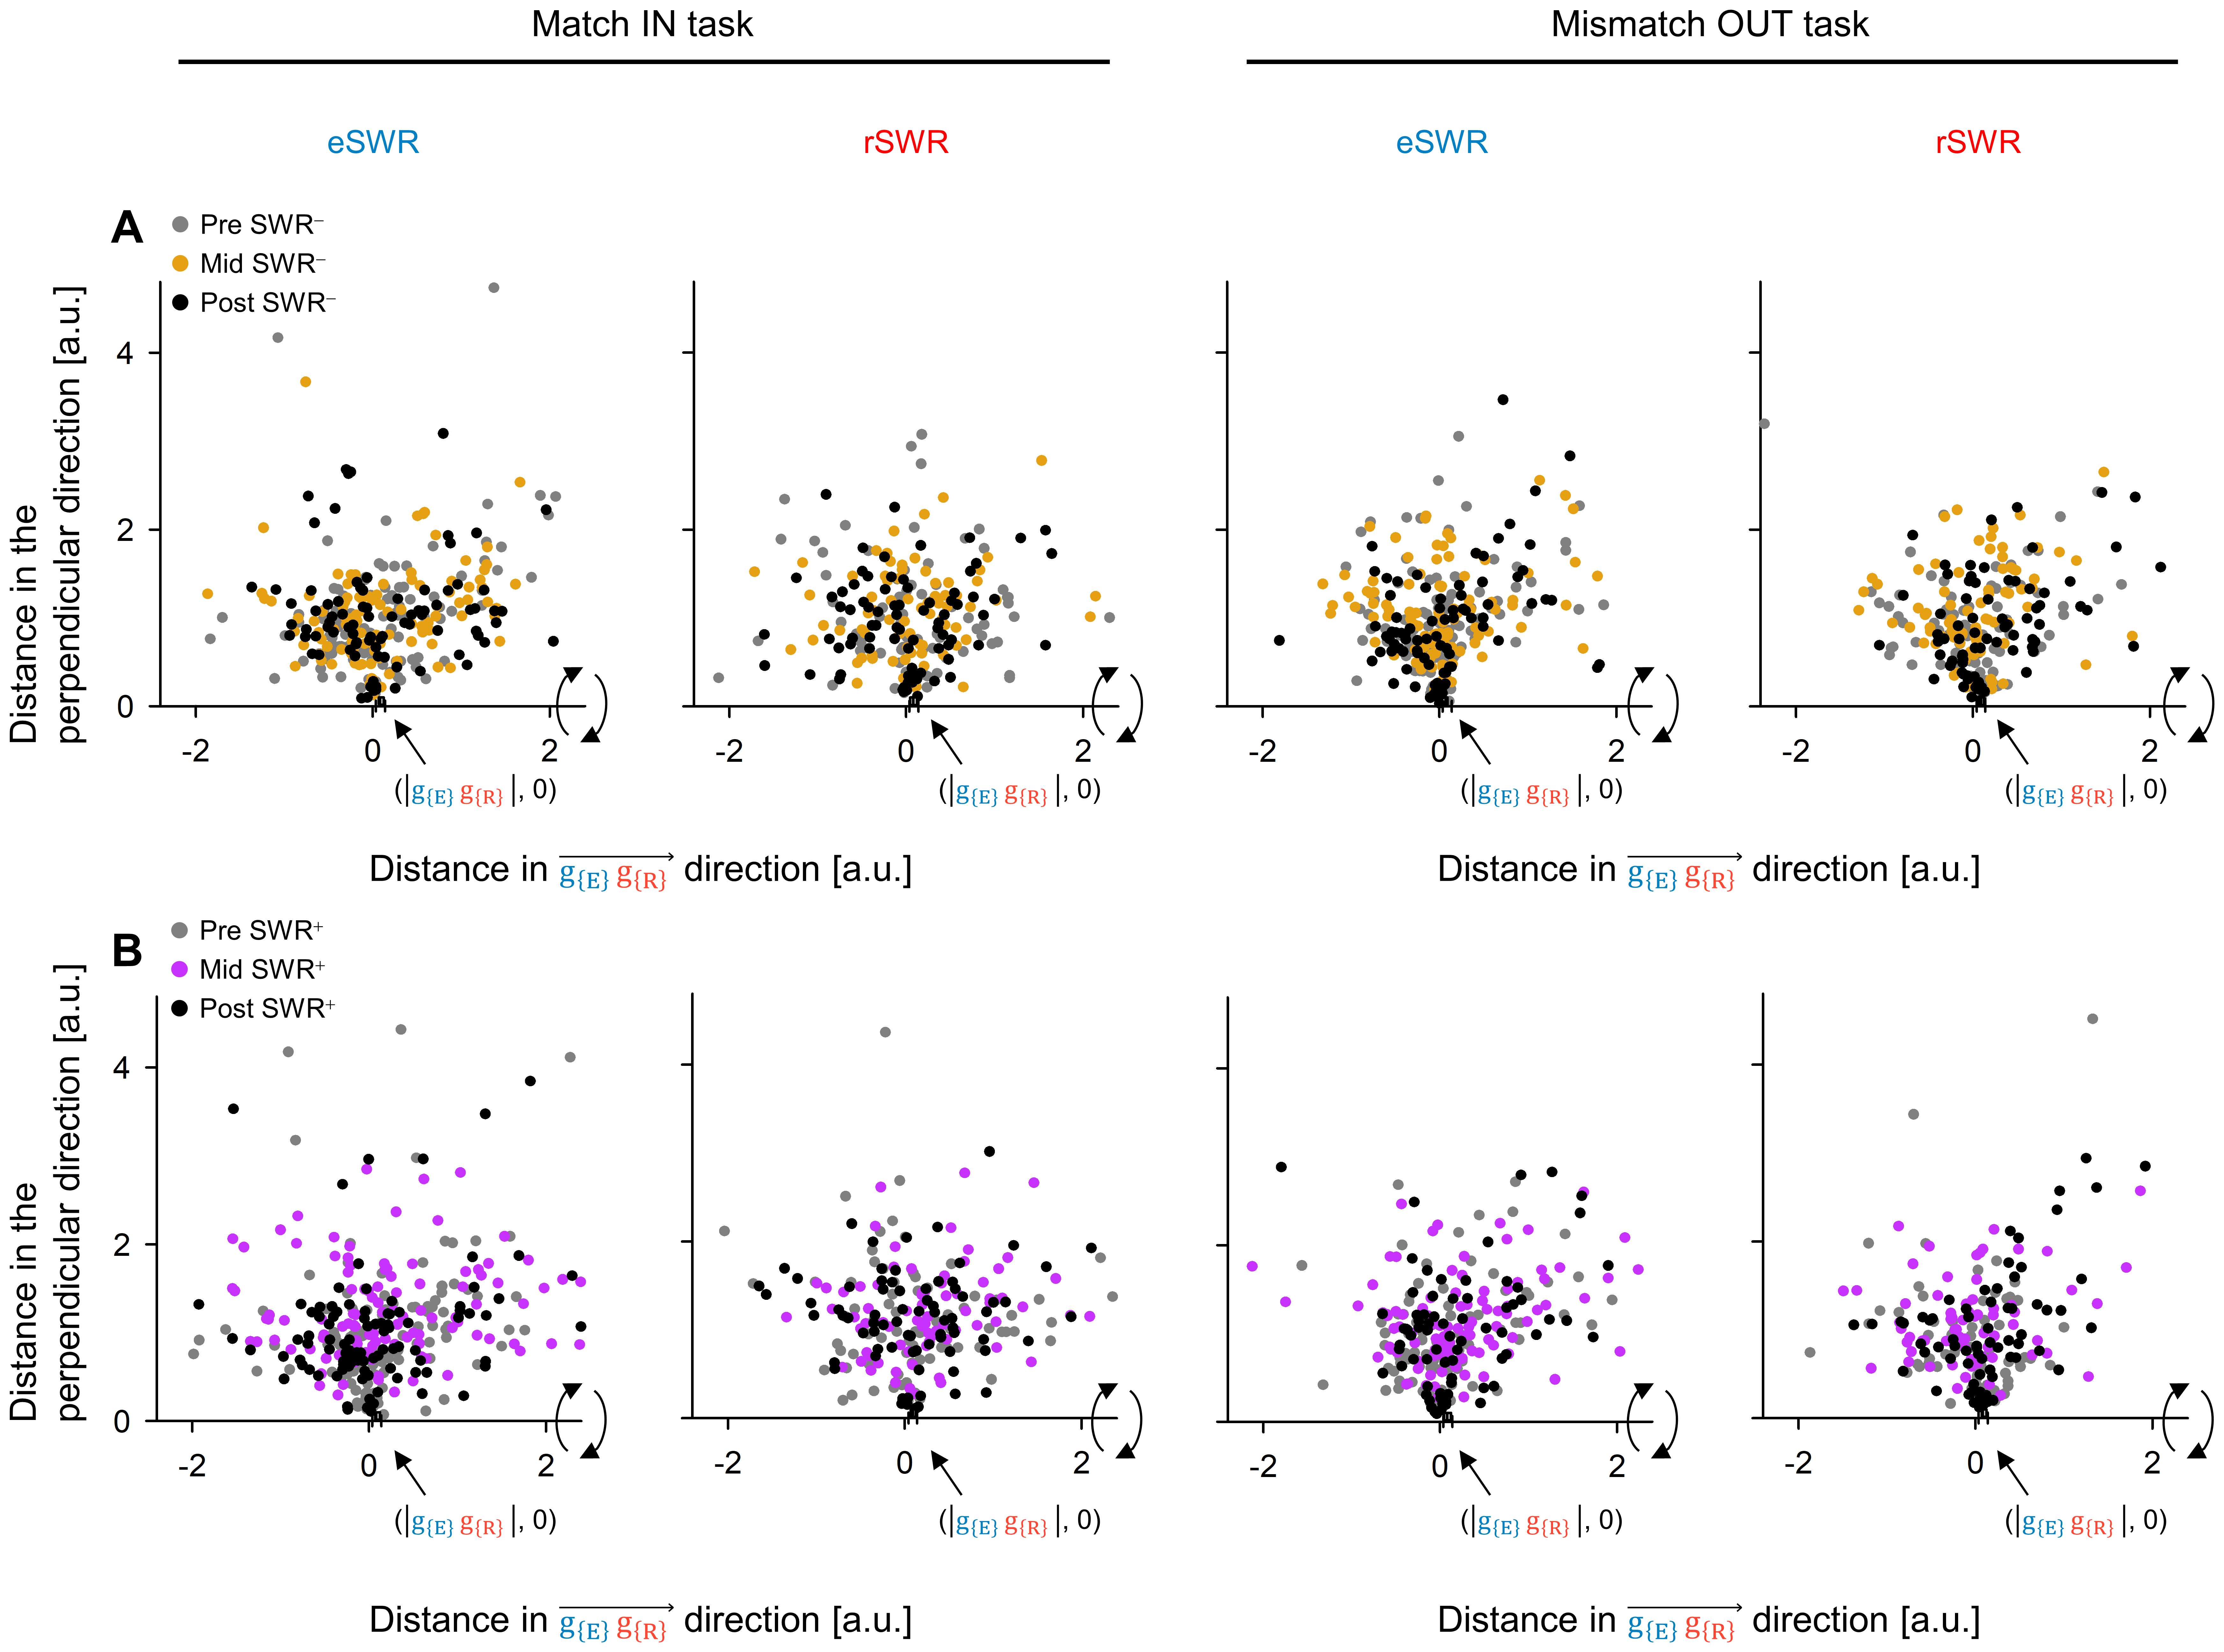
\includegraphics[width=1\textwidth]{./src/figures/.png/Figure_ID_06.png}
        	\caption{\textbf{
Visualizing Neural Trajectories during SWR in Two-Dimensional Spaces}
\smallskip
\\
The figures depict hippocampal neural trajectories during SWR, projected onto two-dimensional spaces. \textbf{\textit{A.}} Displays hippocampal neural trajectories before (pre), during (mid), and after (post) SWR$^-$, denoted in \textit{gray}, \textit{yellow}, and \textit{black}, respectively. \textbf{\textit{B.}} Shows the corresponding trajectories for SWR$^+$. The magnitude of $\lVert \mathrm{g_{E}g_{R}} \rVert$ varied across sessions. The following projection method was employed: Firstly, a linear transformation positioned $\mathrm{g_{E}}$ at origin $O$ (0,0), and $\mathrm{g_{R}}$ at ($\lVert \mathrm{g_{E}g_{R}} \rVert$, 0). The point cloud was then rotated around the $\mathrm{g_{E}g_{R}}$ axis (identical to the x-axis) to fit into the two-dimensional spaces. Consequently, within these two-dimensional spaces, the distances from $O$ and the angles remained consistent with the original properties of the $\mathrm{g_{E}g_{R}}$ axis in the three-dimensional spaces. Abbreviations: SWR refers to sharp-wave ripple events; eSWR represents SWR during the encoding phase; rSWR denotes SWR during retrieval phase; SWR$^+$ indicates an occurrence of SWR event; SWR$^-$ refers to control events for SWR$^+$; pre-SWR, mid-SWR, or post-SWR refer to time intervals from $-800$ to $-250$ ms, from $-250$ to $+250$ ms, or from $+250$ to $+800$ ms from the center of SWR, respectively.}
% width=1\textwidth
        	\label{fig:06}
        \end{figure*}
